\documentclass[12pt,a4paper]{article}
\long\def\/*#1*/{}
\usepackage{verbatim}


\usepackage{listings,chngcntr}
\usepackage{media9}
\usepackage{hyperref}% http://ctan.org/pkg/hyperref
\usepackage{paralist}
\usepackage{xspace}
\usepackage{enumitem}% http://ctan.o\usepackage{amsfonts}rg/pkg/enumitem
\usepackage{amssymb}
\usepackage{amsmath,amsfonts,bm}
\numberwithin{equation}{section}
\DeclareMathOperator{\di}{d\!}
\newcommand*\Eval[3]{\left.#1\right\rvert_{#2}^{#3}}
\usepackage{amsthm}
\newtheorem{theorem}{Theorem}[section]
\newtheorem{corollary}{Corollary}[theorem]
\newtheorem{definition}[theorem]{Definition}
\newtheorem{proposition}[theorem]{Proposition}
\newtheorem{lemma}[theorem]{Lemma}
\usepackage{url}
\usepackage{algorithm}
\usepackage{algpseudocode}
%\usepackage{indentfirst} % paragraph indentation
\usepackage[percent]{overpic}
\makeatletter
\def\BState{\State\hskip-\ALG@thistlm}
\makeatother
\usepackage{mathtools}
%\usepackage{fancyhdr}
%\pagestyle{fancy}
\theoremstyle{definition}
\usepackage{float}
\usepackage[utf8]{inputenc}
\usepackage{cleveref}
\crefname{section}{§}{§§}
\Crefname{section}{§}{§§}
\newcommand{\R}{\mathbb{R}}
\newcommand{\reals}{\rR}
\newcommand{\FD}{\mathcal{D}}
 \usepackage{stmaryrd}
 \usepackage{graphicx}
 \usepackage{caption}
 \usepackage{subcaption}
 \usepackage[english]{babel}
\usepackage{color}
\newcommand{\hilight}[1]{\colorbox{yellow}{#1}}
\newcommand{\fakeimage}{{\fboxsep=-\fboxrule\fbox{\rule{0pt}{3cm}\hspace{4cm}}}}
\usepackage{soul}
\usepackage{tikz}
\usetikzlibrary{hobby,shapes,arrows,fit,calc,positioning} 
\newcommand\restr[2]{{% we make the whole thing an ordinary symbol
		\left.\kern-\nulldelimiterspace % automatically resize the bar with \right
		#1 % the function
		\vphantom{\big|} % pretend it's a little taller at normal size
		\right|_{#2} % this is the delimiter
}}
%\newcommand{\innerprod}[2]{\langle\langle #1,#2\rangle\rangle}}
%\newcommand{\energynorm}[2]{\innerprod{\mathcal{A}^{1/2}#1_1}{arg2}}}
\newcommand{\W}{\ensuremath{\Omega}\xspace}
\newcommand{\dfunkmapsto}[5]{\ensuremath{
		\begin{array}{rccl}
			{#1}: & {#2} &\to&{#3}
			\\
			& {#4} &\mapsto&{#5}
		\end{array}\quad}}
\newcommand{\dfunkmapstonumflux}[5]{\ensuremath{
		\begin{array}{rccl}
			{#1}: & {#2} &\mapsto&{#3}
			\\
			& {#4} &=&{#5}
		\end{array}\quad}}	
\newcommand{\polygs}[3]{\mathbb{P}^{#1}\qp{#2,#3}}
\newcommand{\polygsna}[2]{\mathbb{P}^{#1}\qp{#2}}
\newcommand{\Gs}{\mathbb{R}}
\newcommand{\pnorm}[1]{\left|\left|\left|#1\right|\right|\right|}
\newcommand{\norm}[1]{\left|#1\right|}
\newcommand{\Norm}[1]{\left|\left|#1\right|\right|}
\newcommand{\vect}[1]{\textbf{#1}}
\newcommand{\leb}{\text{L}}
\newcommand{\Coeta}{C_{\overline{\eta}}}
\newcommand{\Cof}{C_{\overline{f}}}
\newcommand{\Cueta}{C_{\underline{\eta}}}
\newcommand{\innerprod}[1]{\langle\langle#1\rangle\rangle}
\newcommand{\innerprodsingle}[1]{\langle#1\rangle}
%\newcommand{\innerprod2}[1]{\langle\langle#1\rangle\rangle}
\newcommand{\rP}{\ensuremath{\mathbb P}\xspace}
\newcommand{\poly}[1]{\ensuremath{\rP}^{#1}}
\newcommand{\qp}[1]{\left(#1\right)}
\newcommand{\qpb}[1]{\left(#1\right]}
\newcommand{\qb}[1]{\left[#1\right]}
\newcommand{\rec}[1]{\widehat{{#1}}}
\newcommand{\rects}[1]{\widehat{{\vect{#1}}}^{ts}}
\newcommand{\rect}[1]{\widehat{{\vect{#1}}}^{t}}
\newcommand{\Normgs}[1]{\left|\left|#1\right|\right|}
\newcommand{\bracegs}[1]{\left\lbrace#1\right\rbrace}
\usepackage{listings}
\usepackage{color}
\usepackage{graphicx, epstopdf}
\usepackage{listings}
\lstset{language=Python}
\renewcommand{\sectionautorefname}{\S}
\setlength{\topmargin}{0.0in}
\setlength{\oddsidemargin}{0.33in}
\setlength{\textheight}{9.0in}
\setlength{\textwidth}{6.0in}
\renewcommand{\baselinestretch}{1.25}
\newtheorem{Defn}[subsection]{Definition}
\newtheorem{Thm}[subsection]{Theorem}
\newtheorem{Proposition}[subsection]{Proposition}
\newtheorem{Lemma}[subsection]{Lemma}
\newtheorem{Rem}[subsection]{Remark}
\newtheorem{Example}[subsection]{Example}
%\linespread{1.3}
\setlist[itemize]{noitemsep, topsep=0pt}
\definecolor{codegreen}{rgb}{0,0.6,0}
\definecolor{codegray}{rgb}{0.5,0.5,0.5}
\lstset{
	frame=single,
	numbers = left,
	basicstyle=\fontsize{9}{11}\ttfamily\linespread{0.85}\ttfamily,
    breaklines=true
}
\setlength{\parindent}{0pt}


\begin{document}
	\begin{titlepage} % Suppresses headers and footers on the title page
		\centering % Centre everything on the title page
		\scshape % Use small caps for all text on the title page
	%	\vspace*{\baselineskip} % White space at the top of the page
		%------------------------------------------------
		%	Title
		%------------------------------------------------
		\rule{\textwidth}{1.6pt}\vspace*{-\baselineskip}\vspace*{2pt} % Thick horizontal rule
		\rule{\textwidth}{0.4pt} % Thin horizontal rule
	%	\vspace{0.75\baselineskip} % Whitespace above the title
		
		{\LARGE Shallow water equations \\Thesis Chapter\\} % Title
		
		\vspace{0.75\baselineskip} % Whitespace below the title
		
		\rule{\textwidth}{0.4pt}\vspace*{-\baselineskip}\vspace{3.2pt} % Thin horizontal rule
		\rule{\textwidth}{1.6pt} % Thick horizontal rule
		
		%\vspace{2\baselineskip} % Whitespace after the title block
		
		%------------------------------------------------
		%	Subtitle
		%------------------------------------------------
	%	A Number of Fascinating and Life-changing Templates Presented in a Clear and Concise Way % Subtitle or further description
		
		%\vspace*{1\baselineskip} % Whitespace under the subtitle
		
		%------------------------------------------------
		%	Editor(s)
		%------------------------------------------------
		

		
		\vspace{0.5\baselineskip} % Whitespace before the editors
		
		{\scshape\Large Author:\\ Georgios Sialounas \\$\,$\\ Supervisor: \\Dr Tristan Pryer} % Editor list
		
	%	\vspace{0.5\baselineskip} % Whitespace below the editor list
		
	%	\textit{The University of Reading\\} % Editor affiliation
		
		\vfill % Whitespace between editor names and publisher logo
		
		
		%------------------------------------------------
		%	Publisher
		%------------------------------------------------
		
		\begin{figure}[H]
			\begin{subfigure}[b]{.15\linewidth}
				
\includegraphics[width=\linewidth]{../figures/icl_logo_big}
			%	\caption{Velocity in $L^2$: $\left|\left|u-u_h\right|\right|_{L^2}$.}
				\label{icl_logo_big}
			\end{subfigure}
			\begin{subfigure}[b]{.1263\linewidth}
				
\includegraphics[width=\linewidth]{../figures/uor_logo_big}
			%	\caption{Velocity in $H^1$: $\left|\left|u-u_h\right|\right|_{H^1}$.}
				\label{uor_logo_big}
			\end{subfigure}
			\centering
		\end{figure}
	\vspace{-14mm}
		\begin{figure}[H]
			\includegraphics[width=.3\linewidth]{../figures/mpe_cdt_logo}
			\centering
		\end{figure}
		\vfill % Whitespace between editor names and publisher logo
		\textit{Report on SHW\\} % Editor affiliation
		31 August, 2018 % Publication year
		
		%{\large publisher} % Publisher
		
	\end{titlepage}
\pagebreak
\thispagestyle{empty}
\emph{I confirm that this is my work and that it has not been submitted for a degree at another university or institution.\\}
\emph{\\}
\emph{\\}
	\vspace{1\baselineskip} 
\text{Georgios Sialounas}
\pagebreak
\pagebreak
\thispagestyle{empty}
\tableofcontents
\section{Introduction}\label{sec_intro}
In this chapter we apply model and mesh adaptivity to the shallow water equations. The aim will be to enable the adaptive introduction and removal of layers of fluid based on an a posteriori error indicator.  The rest of the chapter is as follows.
\section{Preliminaries and Model Setup}\label{sec:setup}
\subsection{Notation}\label{subsec_modelprob}
In this section we present the notation we will be using as well as the model problem.  Let $\qb{0,L}$, $L\in \mathbb{R}^+$ and $t\in \qb{0,T}$ with $T\in \mathbb{R}^+$.  We define the vector of conserved quantities $\vect{u}$  where
\begin{equation}\label{eq_defn_u_multi_d}
\dfunkmapsto{\textbf{u}}{\mathbb{R}\times\mathbb{R}^+}{\mathbb{R}^2}{\qp{x,t}}{\vect{u}\qp{x,t}}
\end{equation}
and the flux function $\vect{f}$
\begin{equation}
\dfunkmapsto{\textbf{f}}{\mathbb{R}^2}{\mathbb{R}^2}{\vect{u}\qp{x,t}}{\vect{f}\qp{\vect{u}\qp{x,t}}}
\end{equation}
Since the Shallow Water Equations (SWE) are a nonlinear conservation law, we define a general framework which we will later use to specify our model problem.
\begin{Rem}[General Multidimensional Scalar conservation law] We consider one dimensional conservation laws, which are of the form
	\begin{equation}\label{eq_gen_hyp_conservation_law}
	\begin{aligned}
	\partial_t \vect{u}\qp{{x},t}+\partial_x{ \vect{f}\qp{\vect{u}\qp{ x,t}}}&=0\\
	\vect{u}\qp{ x,0}&=\vect{u}_0\qp{ {x}},
	\end{aligned}
	\end{equation}
\end{Rem}
\subsection{Model Problem}
In the present work we are concerned with the numerical simulation of the Shallow Water Equations (SWE).  We will define the variables we will work with before formally defining our model problem.
\begin{Rem}[Definition of variables for the SWE]
We define the surface elevation,  $h$, the velocity, $v$, and the discharge, $q:=hv$, of the flow in a domain $\qb{0,L}\times\R^+$ as follows:
\begin{equation}\label{eq_defn_SWE_height}
\dfunkmapsto{h}{\mathbb{R}\times\mathbb{R}^+}{\mathbb{R}^+}{\qp{x,t}}{h\qp{x,t}}
\end{equation}
\begin{equation}\label{eq_defn_SWE_velocity}
\dfunkmapsto{v}{\mathbb{R}\times\mathbb{R}^+}{\mathbb{R}}{\qp{x,t}}{v\qp{x,t}}
\end{equation}
\begin{equation}\label{eq_defn_SWE_discharge}
\dfunkmapsto{q}{\mathbb{R}^+\times\mathbb{R}}{\mathbb{R}}{\qp{h\qp{x,t},v\qp{x,t}}}{h\qp{x,t}v\qp{x,t}}
\end{equation}
\end{Rem}



\begin{Rem}[Shallow Water Equations (SWE) in one spatial dimension] We use the notation from (\ref{eq_gen_hyp_conservation_law}) to formulate the shallow water equations with periodic boundary conditions as follows:
	\begin{equation}
	\begin{aligned}
	\vect{u}=\qp{\begin{array}{c}
h\\
q
		\end{array}}
	\end{aligned}
	\end{equation}
	and 
	\begin{equation}
\begin{aligned}
\vect{f}=\qp{\begin{array}{c}
	hv\\
	hv^2+\frac{1}{2}gh^2
	\end{array}}
\end{aligned}
	\end{equation}
		 Our model problem is given by
\begin{equation}\label{eq_model_SWE}
\begin{aligned}
\begin{array}{c}
h_t\\
q_t
\end{array}
\begin{array}{c}
+\\
+
\end{array}
\begin{array}{c}
\qp{q}_x\\
\qp{hv^2+\frac{1}{2}gh^2}_x
\end{array}
\begin{array}{c}
=0\\
=0,
\end{array}
\end{aligned}
\end{equation}
equipped with the initial conditions
\begin{equation}
\begin{aligned}
h\qp{x,t}&=h_0\qp{x}\\
v\qp{x,t}&=v_0\qp{x},
\end{aligned}
\end{equation}
where $h_0, v_0\in \leb_\infty\qp{\qb{0,L}}$ and with periodic boundary conditions.
\end{Rem}

\subsection{Numerical Discretization}
\begin{Rem}[Discretization of temporal interval]
	We  partition the temporal interval $\qb{0,T}$ into sub-intervals with endpoints given by $0=t^0<t^1<\cdots<t^N=T,\, N\in \mathbb{N}$.    The time-step size is defined by $\Delta t^n:=t^{n+1}-t^n,\, n=0,\cdots,N-1$.    We will use a constant time-step $\Delta t^n=\Delta t \quad \forall n\in \bracegs{0,\cdots, N-1}$.
\end{Rem}
\begin{Rem}[Discretization of spatial domain]
We partition the spatial interval $\W=\qb{0,L}$ into sub-intervals with endpoints given by $0=x_0<x_1<\cdots<x_M=L,\, M\in \mathbb{N}$.  The spatial-step size  defined by $\Delta x_m:=x_{m+1}-x_m,\, m=0,\cdots,-1$.   We will use a constant spatial-step  $\Delta x_j =\Delta x \quad \forall j\in \bracegs{0,\cdots,M-1}$.
\end{Rem}
\subsection{Numerical schemes}
In this section we describe the approximations to the temporal and spatial derivatives from (\ref{eq_gen_hyp_conservation_law}).  
\begin{Rem}[Numerical approximation of $\vect{u}$]  We denote by $\vect{U}^n_j=\qp{H^n_j, Q^n_j}$ the numerical approximation to $\vect{u}\qp{x_j,t^n}=\qp{h\qp{x_j,t^n},q\qp{x_j,t^n}}$.  $\vect{U}^n_j$ will be produced by the numerical schemes we will describe in this section.  
\end{Rem}
\subsubsection{Spatial Approximation}
\begin{Rem}[Spatial Approximation]
We use the shorthand $\vect{f}_h$ to denote a spatial discretization of $\partial_x\vect{f}$ in (\ref{eq_gen_hyp_conservation_law}) i.e
\begin{equation}
\vect{f}_h\qp{\vect{U}^n_j}\approx\partial_x\vect{f}\qp{\vect{u}\qp{x,t}}
\end{equation}
The approximation $\vect{f}_h$ will be defined in  conservative form (see \cite[\S12]{leveque1992numerical}) using a consistent numerical flux function $\vect{F}$ of $p+q+1$ arguments such that
\begin{equation}\label{eq_defn_num_flux}
\dfunkmapstonumflux{\qp{\vect{U}^n_{j-p+1},\cdots,\vect{U}^n_{j+q}}}{\vect{F}^n_j}{\vect{F}\qp{\vect{U}^n_{j-p},\cdots,\vect{U}^n_{j+q}}}{\vect{F}\qp{\vect{v},\cdots,\vect{v}}}{\vect{f}\qp{\vect{v}}}.
\end{equation}
Then, letting $\vect{f}^n_{j,h}$ denote the value of $\vect{f}_h$ at $\qp{x_j, t^n}$ the relation between $\vect{f}_h$ and $\vect{F}$ is given by 
\begin{equation}
\vect{f}^n_{j,h}=\frac{1}{\Delta x}\qp{{\vect{F}\qp{\vect{U}^n_{j-p},\cdots,\vect{U}^n_{j+q}}}-{\vect{F}\qp{\vect{U}^n_{j-p-1},\cdots,\vect{U}^n_{j+q-1}}}}
\end{equation}
\end{Rem}
\subsubsection{Temporal Approximation}
We approximate the temporal derivative $\partial_t\vect{u}$ using Strong-Stability Preserving (SSP) methods (see \cite{gottlieb2001strong}).  These methods were originally developed in \cite{shu1988total} and \cite{shu1988efficient}.  The idea behind them, as explained in \cite{gottlieb2001strong}, is firstly to assume that the forward Euler discretization of the method of lines ODE is strongly stable (TVD stable) under a suitable norm and to then find a higher-order time discretization which maintains this stability, perhaps with a different time-step.

\begin{Rem}[SSP-RK methods]
We will use the SSP methods  from \cite{shu1988total} for the temporal of component  of the discretization. As an illustrative example consider the $3-$stage SSP RK method ($\vect{U}^{\qp{i}}$ refers to the $i^{th}-$stage):
\begin{equation}
\begin{aligned}
\textbf{U}^{\qp{0}}&=\textbf{U}^n,\\
\textbf{U}^{\qp{1}}&=\textbf{U}^n-\Delta t \vect{f}_h\qp{\textbf{U}^{\qp{0}}},\\
\textbf{U}^{\qp{2}}&=\frac{3}{4}\textbf{U}^n +\frac{1}{4}\textbf{U}^{\qp{1}} -\frac{1}{4}\Delta t \vect{f}_h\qp{\textbf{U}^{\qp{1}}},\\
\textbf{U}^{n+1}&=\frac{1}{3}\textbf{U}^n +\frac{2}{3}\textbf{U}^{\qp{2}} -\frac{2}{3}\Delta t \vect{f}_h\qp{\textbf{U}^{\qp{2}}},\\
\end{aligned}
\end{equation}
\end{Rem}

\begin{Rem}[Example of a conservative form using Lax-Friedrichs]
	As an example suppose that we want to use the Lax-Friedrichs (LxF) method for the spatial discretization, coupled with a forward Euler time-stepping scheme. The numerical flux, $\vect{F}$ is given by:
	\begin{equation}\label{eq_F_Lxf_conservative}
	\vect{F}\qp{\vect{U}_j, \vect{U}_{j+1}}=\frac{\Delta x}{2\Delta t}\qp{\vect{U}^n_j-\vect{U}^n_{j+1}}+\frac{1 }{2}\qp{f\qp{\vect{U}_{j}}+f\qp{\vect{U}_{j-1}}}.
	\end{equation}
	This gives us the conservative form of $\vect{f}_h$ as
	\begin{equation}
	\vect{f}^n_{h,j}= \frac{1}{\Delta x}\qp{\vect{F}\qp{\vect{U}^n_j, \vect{U}^n_{j+1}}-\vect{F}\qp{\vect{U}^n_{j-1}, \vect{U}^n_{j}}}
	\end{equation}
	and the Forward Euler-Lax-Friedrichs scheme as 
	\begin{equation}
	\vect{U}^{n+1}_j=\vect{U}^n_j-\Delta t\vect{f}^n_{h,j}.
	\end{equation}
\end{Rem}

\section{Reconstructions and a-posteriori bounds}\label{sec_bounds}
In this section we develop reconstructions for numerical solutions to (\ref{eq_model_SWE}).  Then, we use the reconstructions to obtain an a posteriori error bound for the error of the numerical scheme.  

\begin{Rem}[Reconstruction procedure]
We reconstruct firstly in time and then in space as the temporal component of (\ref{eq_gen_hyp_conservation_law}) is linear whereas the spatial one may contain nonlinearities, as it does for SWE.
\end{Rem}
\begin{Defn}[Space of the spatial component of the reconstruction]
Let $\polygsna{q}{\qb{x_j, x_{j+1}}}$  denote the space of polynomials of degree $q\in\mathbb{N}$ over the sub-interval $\qb{x_j, x_{j+1}}$.  We define the space of the spatial component of the reconstruction 
\begin{equation}
\mathbb{V}_q^s:=\bracegs{w:\qb{0,L}\rightarrow\mathbb{R}: w|_{\qb{x_j,x_{j+1}}}\in \polygsna{q}{\qb{x_j, x_{j+1}}}}
\end{equation}
to be the space of piecewise polynomials of degree $q$ over $\qb{0,L}$.  We use the superscript $s$ to indicate that this space pertains to the spatial component of the reconstruction.
\end{Defn}

\begin{Defn}[Space of the temporal reconstruction]
 Let $V$ denote a temporary spaceholder for the spatial component of the reconstruction. We formally define the space of the temporal reconstruction as the space of piecwise polynomials of degree $r$ over $\qb{0,T}$ such that
\begin{equation}
\mathbb{V}_r^t\qp{\qb{0,T}}:=\bracegs{g:\qb{0,T}\rightarrow V: g|_{\qb{t^n, t^{n+1}}}\in \polygsna{q}{\qb{t^n, t^{n+1}}}}.
\end{equation}
\end{Defn}
 

\begin{Defn}[Temporal reconstruction]\label{defn_temp_rec_shw}
The temporal reconstruction of the numerical solution $\vect{U}$ of (\ref{eq_gen_hyp_conservation_law}) of (\ref{eq_model_SWE}), is the function $ \widehat{\textbf{U}}^t=\qp{ \widehat{h}, \widehat{q}}\in \mathbb{V}_r^t\qp{\qb{0,T}}$ satisfying 
\begin{equation}\label{eq_temp_rec_conds}
\begin{aligned}
 \widehat{\textbf {U}}_j^t\qp{t^n}&={\textbf{U}}^n_j\quad \text{and}\\
\partial_t \widehat{\textbf{U}}_j^t\qp{t^n}&=-\vect{f}_{h,j}^n,
\end{aligned}
\end{equation}
for $j=0,\cdots,M$
\end{Defn}
\begin{Rem}[Polynomial form of the temporal reconstruction] The conditions (\ref{eq_temp_rec_conds}) can be used to obtain $\rect{U}$as a polynomial in $\qp{t-t^n}$:
	\begin{equation}
		\widehat{\textbf {U}}^t\qp{t}:=\vect{c}_0 +\vect{c}_1\qp{t-t^n} +\vect{c}_2\qp{t-t^n}^2+\vect{c}_3\qp{t-t^n}^3,
	\end{equation}
where the coefficients $\vect{c}_i$ are as follows:
	\begin{equation}
	\begin{aligned}
	\vect{c}_{0} &= \vect{U}^n\\
	\vect{c}_{1}&=-\vect{f}_h\qp{\vect{U}^n} \\
	\vect{c}_{2}&=\frac{1}{\Delta t}\qp{\vect{f}_h\qp{\vect{U}^{n+1}}-\vect{f}_h\qp{\vect{U}^{n}}}+\frac{3}{\Delta t^2}\qp{\vect{U}^{n+1}-\vect{U}^{n}+\Delta t \vect{f}_h\qp{\vect{U}^n}}\\
	\vect{c}_{3}&=-\frac{1}{\Delta t^2}\qp{\vect{f}_h\qp{\vect{U}^{n+1}}-\vect{f}_h\qp{\vect{U}^{n}}}-\frac{2}{\Delta t^3}\qp{\vect{U}^{n+1}-\vect{U}^{n}+\Delta t \vect{f}_h\qp{\vect{U}^n}}\\
	\end{aligned}
	\end{equation}
\end{Rem}

We now use the temporal reconstruction to obtain the spatio-temporal one.  In order to define the full spatio-temporal reconstruction we will need to make use of difference quotients to approximate the derivatives of $\vect{u}$.  
\begin{Defn}[Finite difference approximation of deratives of \vect{u}]
We will use the notation 
$\FD\qp{\vect{U}^n_j}$
to denote the chosen finite difference approximation to $\partial_x\vect{u}\qp{x_j,t^n}$.
\end{Defn}
\begin{Defn}[Spatio-temporal reconstruction]\label{defn_spatio-temporal reconstruction}
	Let $ \widehat{\textbf{U}}^t=\qp{\rec{h}^t,\rec{q}^t}$ be a temporal reconstruction of the numerical solution $\vect{U}$ of (\ref{eq_gen_hyp_conservation_law}).  The spatio-temporal reconstruction $\widehat{\textbf{U}}^{ts}=\qp{\rec{h}^{ts},\rec{q}^{ts}}\in\mathbb{V}^t_r\qp{0,T; \mathbb{V}^s_q}$ is given by
	\begin{equation}\label{eq_conds_spatiotemp}
	\begin{aligned}
	 \widehat{\vect {U}}^{ts}\qp{\vect x_j,t^n}&= 
	{ \widehat{\vect {U}}^t}_j\qp{t^n}\quad \text{and}\\
	\partial_{x}{ \widehat{\vect {U}}^{ts}\qp{\vect x_j,t^n}}&= 
	\FD{\qp{ \widehat{\vect {U}}^t_j  }}
	\end{aligned}
	\end{equation}
	for $  j=0\cdots,M-1$.  
\end{Defn}

\begin{Defn}[Polynomial form of the spatio-temporal reconstruction]\label{defn_spatio_temp_rec_shw}
	The spatio-temporal reconstruction can be obtained as a polynomial in $\qp{x-x_j}$  using the conditions (\ref{eq_conds_spatiotemp}):
	\begin{equation}
\rects{U}\qp{x,t}:=\vect{c}_0\qp{t} +\vect{c}_1\qp{t}\qp{x-x_j} +\vect{c}_2\qp{t}\qp{x-x_j}^2+\vect{c}_3\qp{t}\qp{x-x_j}^3,
	\end{equation}
where the $\vect{c}_i\qp{t}$ are as follows:
	\begin{equation}
	\begin{aligned}
	\vect{c}_{0}\qp{t} &= \rec{\vect{U}}^t_j\qp{t},\\
	\vect{c}_{1}\qp{t}&=\FD\qp{\rec{\vect{U}}^t_j\qp{t}},\\
	\vect{c}_{2}\qp{t}&=-\frac{1}{\Delta x}\qp{\FD\qp{\rec{\vect{U}}_{j+1}\qp{t}}-\FD\qp{\rec{\vect{U}}^t_j\qp{t}}}+
	\frac{3}{\Delta x^2}\qp{ \rec{\vect{U}}^t_{j+1}\qp{t}- \rec{\vect{U}}^t_j\qp{t}-\Delta x\FD\qp{\rec{\vect{U}}^t_{j}\qp{t}}}\quad \text{and}\\
	\vect{c}_{3}\qp{t}&=\frac{1}{\Delta x^2}\qp{\FD\qp{\rec{\vect{U}}^t_{j+1}\qp{t}}-\FD\qp{\rec{\vect{U}}^t_{j}\qp{t}}}
	-\frac{2}{\Delta x^3}\qp{\rec{\vect{U}}^t_{j+1}\qp{t}-\rec{\vect{U}}^t_j\qp{t}-\Delta x \FD\qp{\rec{\vect{U}}^t_j\qp{t}}}.\\
	\end{aligned}
	\end{equation}
\end{Defn}

\subsection{Error equation and estimators}\label{subsec_error_estimators}
In what follows, we drop the superscript $\qp{\cdot}^{ts}$ and we henceforth take $\rec{\vect{U}}$ to be the full spatio-temporal reconstruction $\rects{U}$ defined in \ref{defn_spatio-temporal reconstruction}.
\begin{Defn}[Errors]\label{defn:errors}
We define the reconstruction errors for $\rec{h}$ and $\rec{q}$ as
\begin{equation}\label{eq_err_rec_uv}
\begin{aligned}
 \widehat{e}_h&:=h- \widehat{h}^{ts} \quad \text{and}\\
 \widehat{e}_q&:=q- \widehat{q}^{ts}.
\end{aligned}
\end{equation}
\end{Defn}
This leads us to the form of the residual equations.
\begin{Defn}[Residual equations]
The reconstruction of the numerical solution for (\ref{eq_model_SWE}) satisfies the equations
\begin{equation}\label{eq_residuals}
\begin{aligned}
{\begin{array}{c}
	 \widehat{h}_t\\
	 \widehat{q}_t\\
	\end{array}
}
+
{\begin{array}{c}
	 \widehat{q}_x\\
\qp{	 \rec{h}\rec{v}^2+\frac{1}{2}g \rec{h}^2}_x
	\end{array}
}
{\begin{array}{c}
	=\\
	=
	\end{array}
}
{\begin{array}{c}
	\mathcal{R}_h\\
	\mathcal{R}_q
	\end{array}}\\
\end{aligned}
\end{equation}
where  $\mathcal{R}_{h,q}$ are residuals which depend upon the chosen reconstruction.
\end{Defn}

\begin{Rem}[A-posteriori error bound for (\ref{eq_model_SWE}) from \cite{giesselmann2015posteriori}]\label{thm:bound}
Let $\vect{u}$ be the solution of (\ref{eq_model_SWE}) and $ \widehat{\vect{e}}_u:=\vect{u}-\rec{\vect{U}}$. Then the following a posteriori error estimate holds
\begin{equation}\label{eq_bound}
\begin{aligned}
\Norm{\vect{u}\qp{\cdot,t}- \widehat{\vect{u}}\qp{\cdot,t}}_{\leb_2\qp{I}}^2\leq& C_{\underline{\eta}}^{-1}\qp{\Norm{\vect{R}}^2_{\leb_2\qp{I\times\qp{0,t}}} +C_{\overline{\eta}}\qp{\Norm{\vect{u}_0-\rec{\vect{u}}_0}_{\leb_2\qp{I}}}}\\
&\times\exp\qp{\int^t_0\frac{\Cueta\Cof\Norm{\partial_x\rec{\vect{u}}\qp{\cdot,s}}_{\leb_\infty\qp{I}}+\Coeta^2}{\Cueta}\mathrm{d}s}
\end{aligned}
\end{equation}
where $\vect{R}=\qp{\mathcal{R}_h,\mathcal{R}_q}$, which are defined in (\ref{eq_residuals}).
\end{Rem}

\section{Numerical Experiments}\label{sec_num_exp}
The objectives in this section are to study the performance of the bound given in (\ref{eq_bound}), which we formally define as 
\begin{equation}\label{eq_estimator}
\begin{aligned}
\eta^2:=& C_{\underline{\eta}}^{-1}\qp{\Norm{\vect{R}}^2_{\leb_2\qp{I\times\qp{0,t}}} +C_{\overline{\eta}}\qp{\Norm{\vect{u}_0-\rec{\vect{u}}_0}_{\leb_2\qp{I}}}}\\
&\times\exp\qp{\int^t_0\frac{\Cueta\Cof\Norm{\partial_x\rec{\vect{u}}\qp{\cdot,s}}_{\leb_\infty\qp{I}}+\Coeta^2}{\Cueta}\mathrm{d}s}
\end{aligned}
\end{equation}
The assessment of the performance of the bound will be on the basis of the Effectivity Index (EI) of the error indicators and of the Estimated Order of Convergence (EOC).
\begin{Defn}[Effectivity Index (EI)] The effectivity index of an error indicator $\eta$ compared to a given error at time $t$ is defined as
\begin{equation}\label{eq_EI}
EI\qp{error\qp{t}, \eta\qp{t}} := \frac{\eta_1\qp{t}}{error\qp{t}}
\end{equation}
\end{Defn}

\begin{Defn}[Estimated Order of Convergence (EOC)] Given two sequences $a\qp{i}$ and $h\qp{i}\downarrow 0$, we define the estimated order of convergence as
\begin{equation}
EOC\qp{a,h;i} = \frac{log\qp{a\qp{i+1}/a\qp{i}}}{log\qp{h\qp{i+1}/h\qp{i}}}.
\end{equation}
\end{Defn}

\subsection{Test 1: Smooth initial conditions}  We benchmark the performance of the estimator (\ref{eq_estimator}) for a sinusoidal initial condition:
\begin{equation}
\begin{aligned}
\widehat{h}_0&=	0.2+0.1\sin\qp{\pi x /16}\\
\widehat{q}_0&=0
\end{aligned}
\end{equation}
with periodic boundary conditions. 
\subsection{Test results}\label{sec:num_exp}
In the tests that follows, for the time being, we are just looking at $\Norm{\vect{R}}_{\leb_2}$ \textbf{Put the coupling and the method in the caption and change Rhv to Rq}
\subsection*{$\Delta t \sim \Delta x^1$}
\begin{figure}[H]
	\hspace{-3cm}
	%\centering
	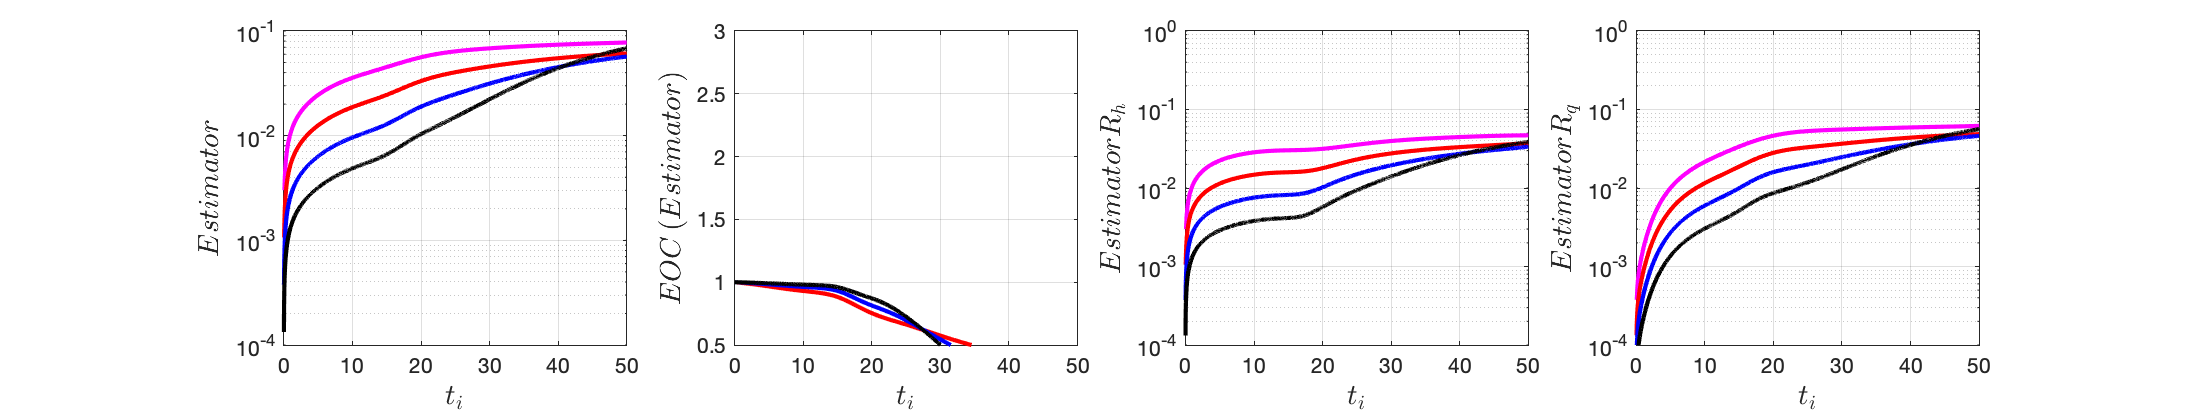
\includegraphics[scale=0.55]{../figures/fig_SHW_RK1_LXF_rec1_pow_oneplots_1x5_shw_periodic}	
	\caption{Reconstruction from Defn. \ref{defn_spatio-temporal reconstruction}. (from left to right) Error $e$ given by (\ref{eq_error_eR}), Estimator $\eta$ given by (\ref{eq_estimator}), EOC error, EOC Estimator, Effectivity Index.}
	\label{fig_all_RK1_LXF_rec1_pow_one}
\end{figure}

\begin{figure}[H]
	\hspace{-3cm}
	%\centering
	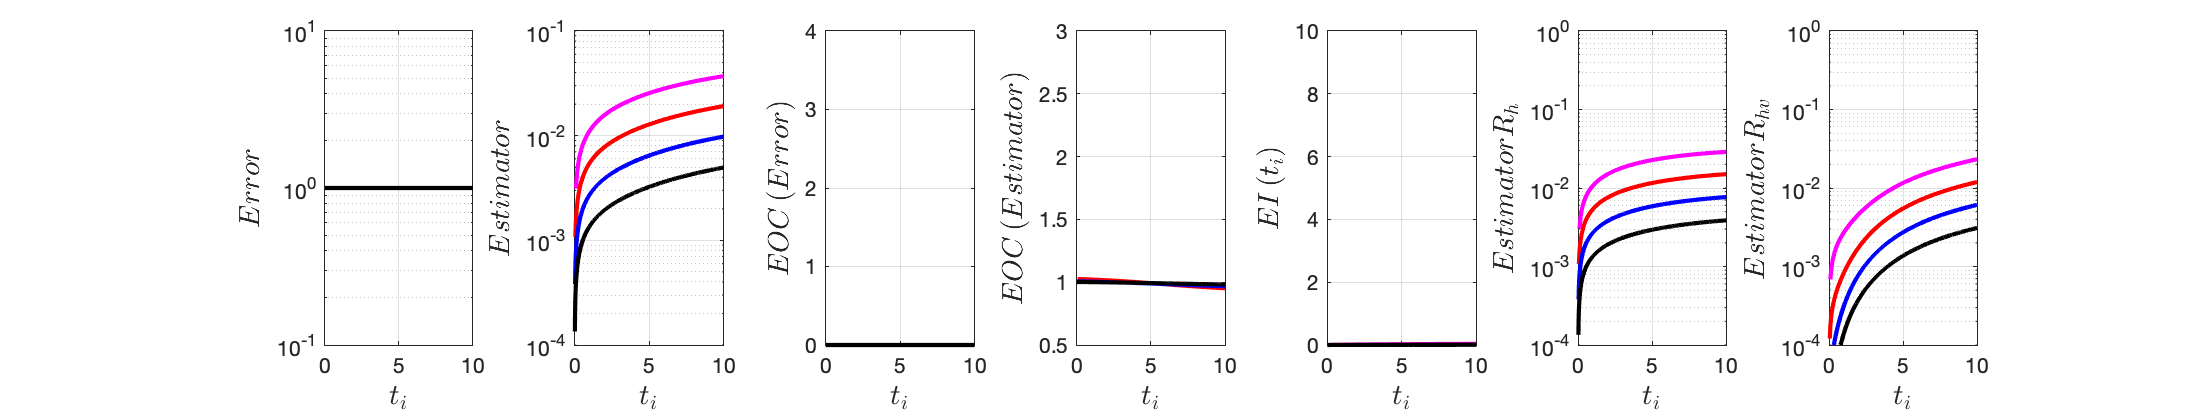
\includegraphics[scale=0.55]{../figures/fig_SHW_RK3_LXF_rec3_pow_oneplots_1x5_shw_periodic}	
	\caption{Reconstruction from Defn. \ref{defn_spatio-temporal reconstruction}. (from left to right) Error $e$ given by (\ref{eq_error_eR}), Estimator $\eta$ given by (\ref{eq_estimator}), EOC error, EOC Estimator, Effectivity Index.}
	\label{fig_all_RK3_LXF_rec3_pow_one}
\end{figure}



\subsection*{$\Delta t \sim \Delta x_{finest}$}
\begin{figure}[H]
	\hspace{-3cm}
	%\centering
	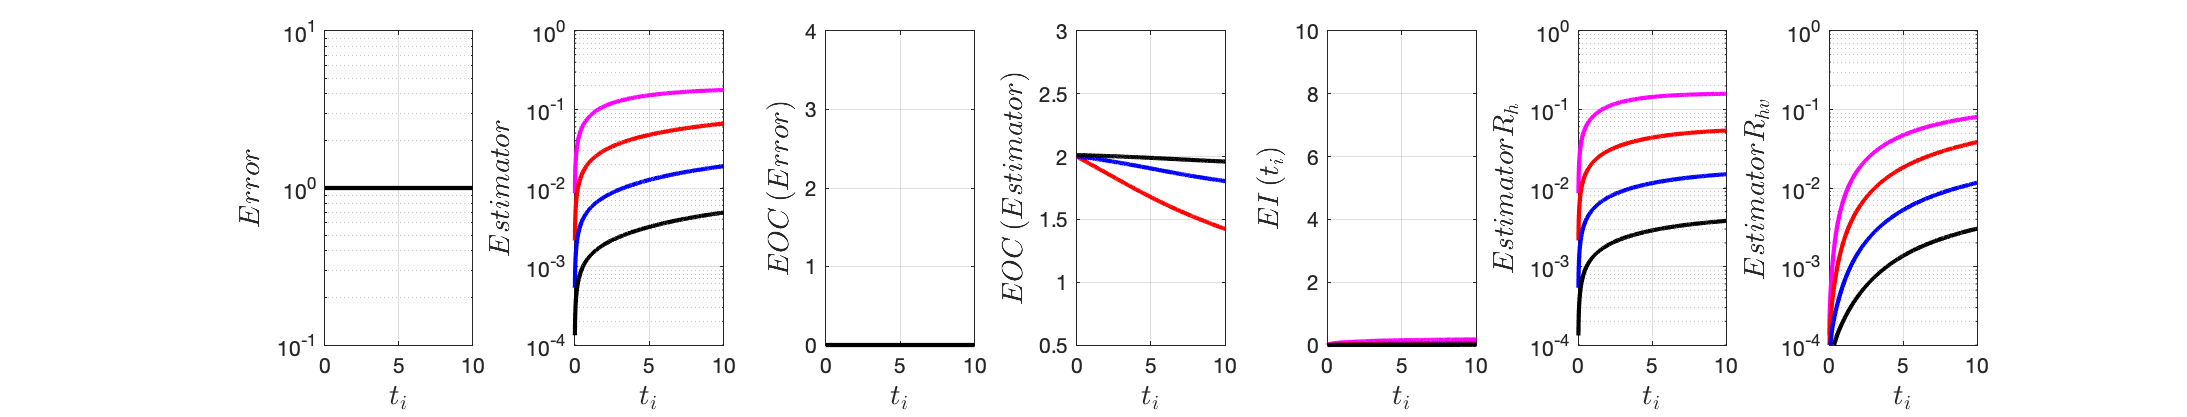
\includegraphics[scale=0.55]{../figures/fig_SHW_RK1_LXF_rec1_fixedplots_1x5_shw_periodic}	
	\caption{Reconstruction from Defn. \ref{defn_spatio-temporal reconstruction}. (from left to right) Error $e$ given by (\ref{eq_error_eR}), Estimator $\eta$ given by (\ref{eq_estimator}), EOC error, EOC Estimator, Effectivity Index.}
	\label{fig_all_RK1_LXF_rec1_fixed}
\end{figure}

\begin{figure}[H]
	\hspace{-3cm}
	%\centering
	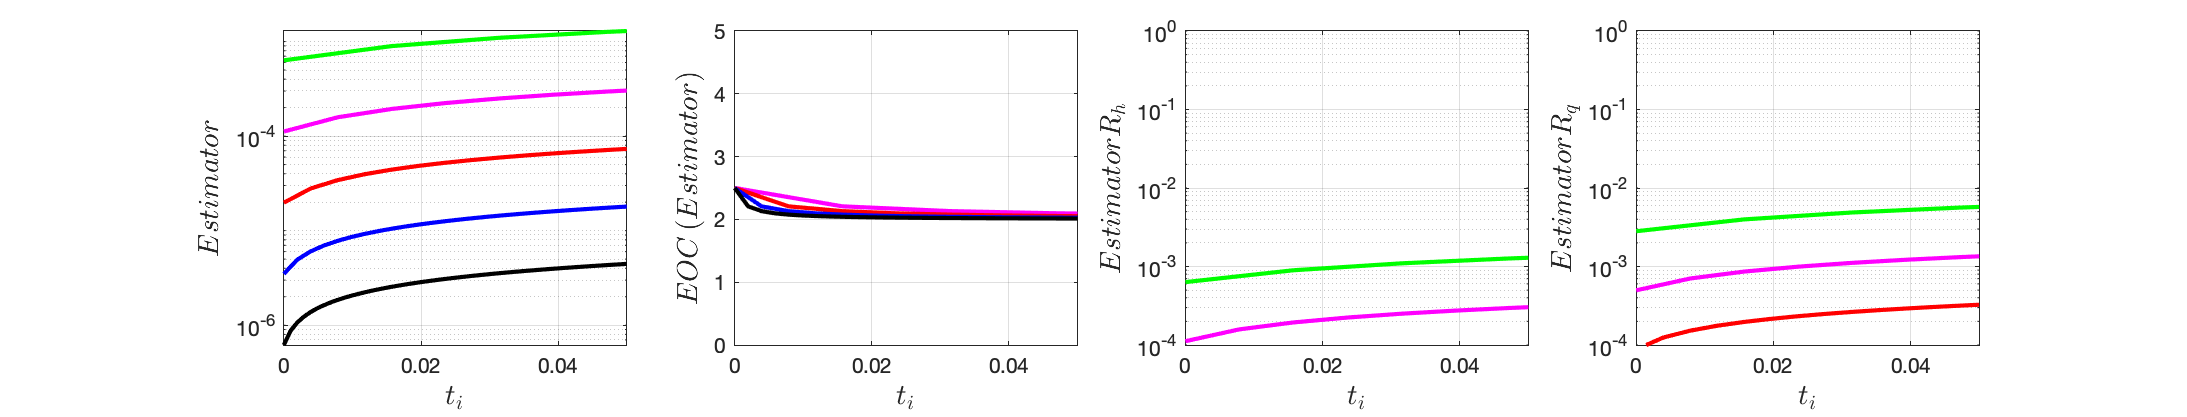
\includegraphics[scale=0.55]{../figures/fig_SHW_RK3_LXF_rec3_fixedplots_1x5_shw_periodic}	
	\caption{Reconstruction from Defn. \ref{defn_spatio-temporal reconstruction}. (from left to right) Error $e$ given by (\ref{eq_error_eR}), Estimator $\eta$ given by (\ref{eq_estimator}), EOC error, EOC Estimator, Effectivity Index.}
	\label{fig_all_RK3_LXF_rec3_fixed}
\end{figure}

\subsection*{$\Delta t \sim \Delta x_{finest}^2$}
\begin{figure}[H]
	\hspace{-3cm}
	%\centering
	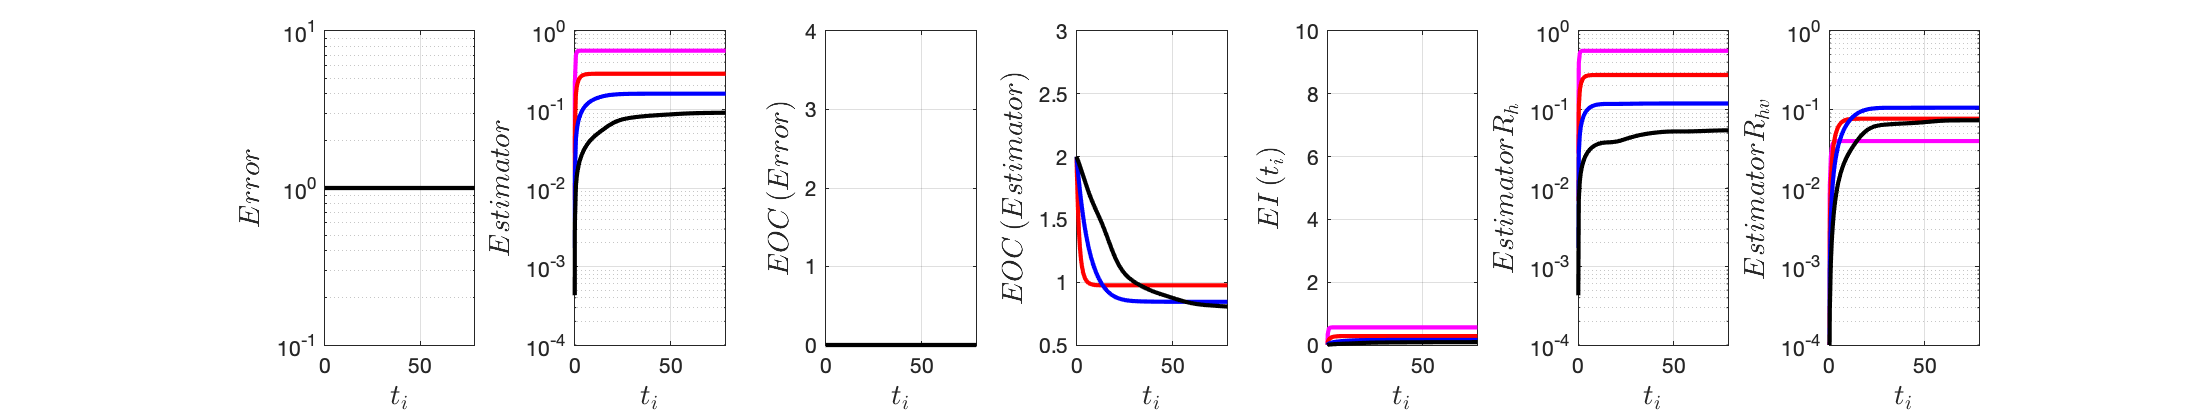
\includegraphics[scale=0.55]{../figures/fig_SHW_RK1_LXF_rec1_pow_twoplots_1x5_shw_periodic}	
	\caption{Reconstruction from Defn. \ref{defn_spatio-temporal reconstruction}. (from left to right) Error $e$ given by (\ref{eq_error_eR}), Estimator $\eta$ given by (\ref{eq_estimator}), EOC error, EOC Estimator, Effectivity Index.}
	\label{fig_all_RK1_LXF_rec1_pow_two}
\end{figure}

\begin{figure}[H]
	\hspace{-3cm}
	%\centering
	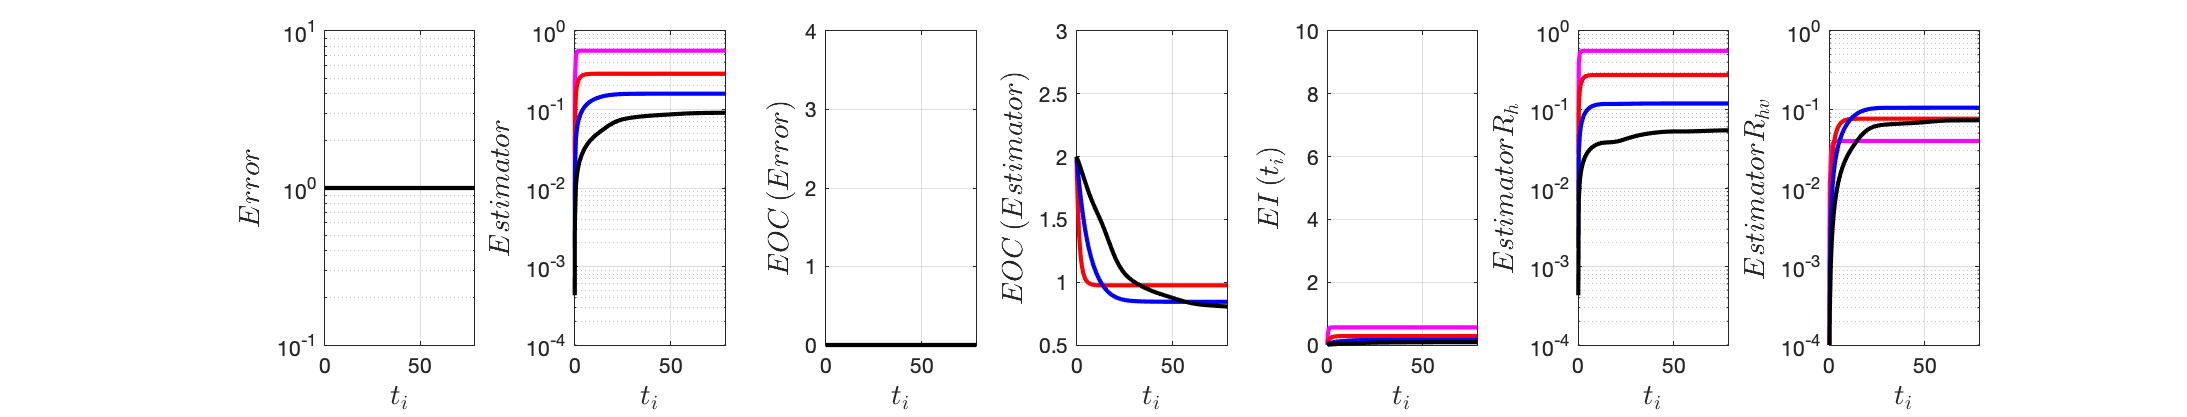
\includegraphics[scale=0.55]{../figures/fig_SHW_RK3_LXF_rec3_pow_twoplots_1x5_shw_periodic}	
	\caption{Reconstruction from Defn. \ref{defn_spatio-temporal reconstruction}. (from left to right) Error $e$ given by (\ref{eq_error_eR}), Estimator $\eta$ given by (\ref{eq_estimator}), EOC error, EOC Estimator, Effectivity Index.}
	\label{fig_all_RK3_LXF_rec3_pow_two}
\end{figure}




\section{Discussion}\label{sec:discussion}

\section{Conclusion}


\bibliography{apostfd_bibdesk}
\bibliographystyle{ieeetr}
\end{document}